\section{Definiciones y resultados previos}
		\begin{frame}{Definiciones Previas}
			\begin{definition} 
				Dada una función $f:\Omega \subseteq \mathbb R^2  \to \mathbb{R}$ continua, una un problema de valores iniciales de primer orden consiste en encontrar aquellas funciones $y: [a,b] \rightarrow \mathbb{R}$ de clase 1 que verifiquen $G(y) \subset \Omega$, $y'(t) = f(t,y(t)) \ \forall t \in [a,b]$ y la condición inicial $y(t_0) = y_0$, donde $t_0 \in [a,b]$.  
			\end{definition}
		
			\begin{definition}
				Sea $\Omega \subset \mathbb{R}^2$ y sea $f : \Omega \rightarrow \mathbb{R}$. Se dice que $f$ es lipschitziana respecto de la segunda variable, $y$, si existe una constante $L \in \mathbb{R^{+}}$, llamada constante de Lipschitz, de forma que $|f(t,y_1) - f(t, y_2)| \le L|y_1 - y_2|$ para cualquier par de puntos $(t,y_1), (t,y_2) \in \Omega$.  
			\end{definition}
		\end{frame}
	
	\subsection*{Funcionamiento de TPCx-HS}	

		\begin{frame}{Funcionamiento de TPCx-HS}
			\begin{tcolorbox}[colback=ChetwodeBlue!10,colframe=ChetwodeBlue!60]
				\fontsize{8}{8}\selectfont
				\centering
				\textbf{Dos ejecuciones de cinco fases cada una.}
			\end{tcolorbox}
			
				\begin{columns}[c]
					\column{.6\textwidth}
						\fontsize{8}{10}\selectfont
											
						\begin{itemize}
							\item Fase 1: Generación de los datos. \\ 3-ways replication
							\item Fase 2: Verificación de la validez de los datos.
							\item Fase 3: Ordenación de los datos.  \\ 3-ways replication
							\item Fase 4: Verificación de la validez de los datos.
							\item Fase 5: Validación de la salida
						\end{itemize}
					
					\column{.4\textwidth}
						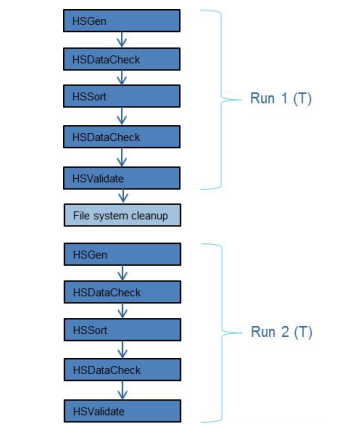
\includegraphics[width=\textwidth]{./Images/executionsTPC.png}
				\end{columns}
	
		\end{frame}
		
	\subsection*{Medida del rendimiento}	
			
		\begin{frame}{Rendimiento}		
			
			{\color{ChetwodeBlue}\large Medida del rendimiento.}
								
					$$ HSph@SF = \frac{SF}{T/3600} $$				
				
			{\color{ChetwodeBlue}\large Medida del rendimiento-precio.}
			
					$$ \$/HSph@SF = \frac{P}{HSph@SF} $$
					
			\begin{tcolorbox}[colback=blue!5,colframe=blue!15]
				\textbf{Parámetros:}
		
				\begin{itemize}
					\fontsize{10}{10}\selectfont
					\item SF: factor de escala escogido.
					\item T: tiempo total de las dos ejecuciones.
					\item P: costo del sistema bajo estudio.
				\end{itemize}
			\end{tcolorbox}
		\end{frame}
				 